\documentclass[a4paper]{scrreprt}

%% Language and font encodings
\usepackage[english]{babel}
\usepackage[utf8x]{inputenc}
\usepackage[T1]{fontenc}

%% Sets page size and margins
\usepackage[a4paper,top=3cm,bottom=2cm,left=3cm,right=3cm,marginparwidth=1.75cm]{geometry}

%% Useful packages
\usepackage{amsmath}
\usepackage{graphicx}
\graphicspath{ {./img/} }
\usepackage[colorinlistoftodos]{todonotes}
\usepackage[colorlinks=true, allcolors=blue]{hyperref}

\title{Hattori}
\subtitle{"A vertical scrolling space-shooter"}
\author{Edward Eldridge (G00337490)}
\titlehead{\centering
\includegraphics[width=15cm]{HattoriLogo}}


\begin{document}
\maketitle

\begin{abstract}

  Hattori aim's to be a top-down vertical scrolling shooter taking inspiration from games such as Galaga, Space Invaders and Ikagura.
  Expanding on the core mechanic of these games, Hattori aim's to
  add a new layer of depth to these games by introducing an in-depth resource management system combined with new and exciting weapon upgrades for your ship. 

\end{abstract}

{
  \hypersetup{linkcolor=black}
  \tableofcontents
}

% ______________________
% chapter Overview
% ______________________
\chapter{Overview}

Hattori aim's to be a top-down vertical scrolling shooter taking inspiration from games such as Galaga, Space Invaders and Ikagura.
Expanding on the core mechanic of these games, Hattori aim's to
add a new layer of depth to these games by introducing an in-depth resource management system combined with new and exciting weapon upgrades for your ship. 

% ______________________
% chapter References
% ______________________

\chapter{References} 
Ikaruga

% ______________________
% chapter Specification and Market Analysis 
% ______________________

\chapter{Specification}

\section{Genre}
The game will be vertical-scrolling shooter.


\section{Art Style}
The art style of the game will be mainly sci-fi/space focused but will take inspiration from Eastern culture and art. 
\begin{figure}
\centering
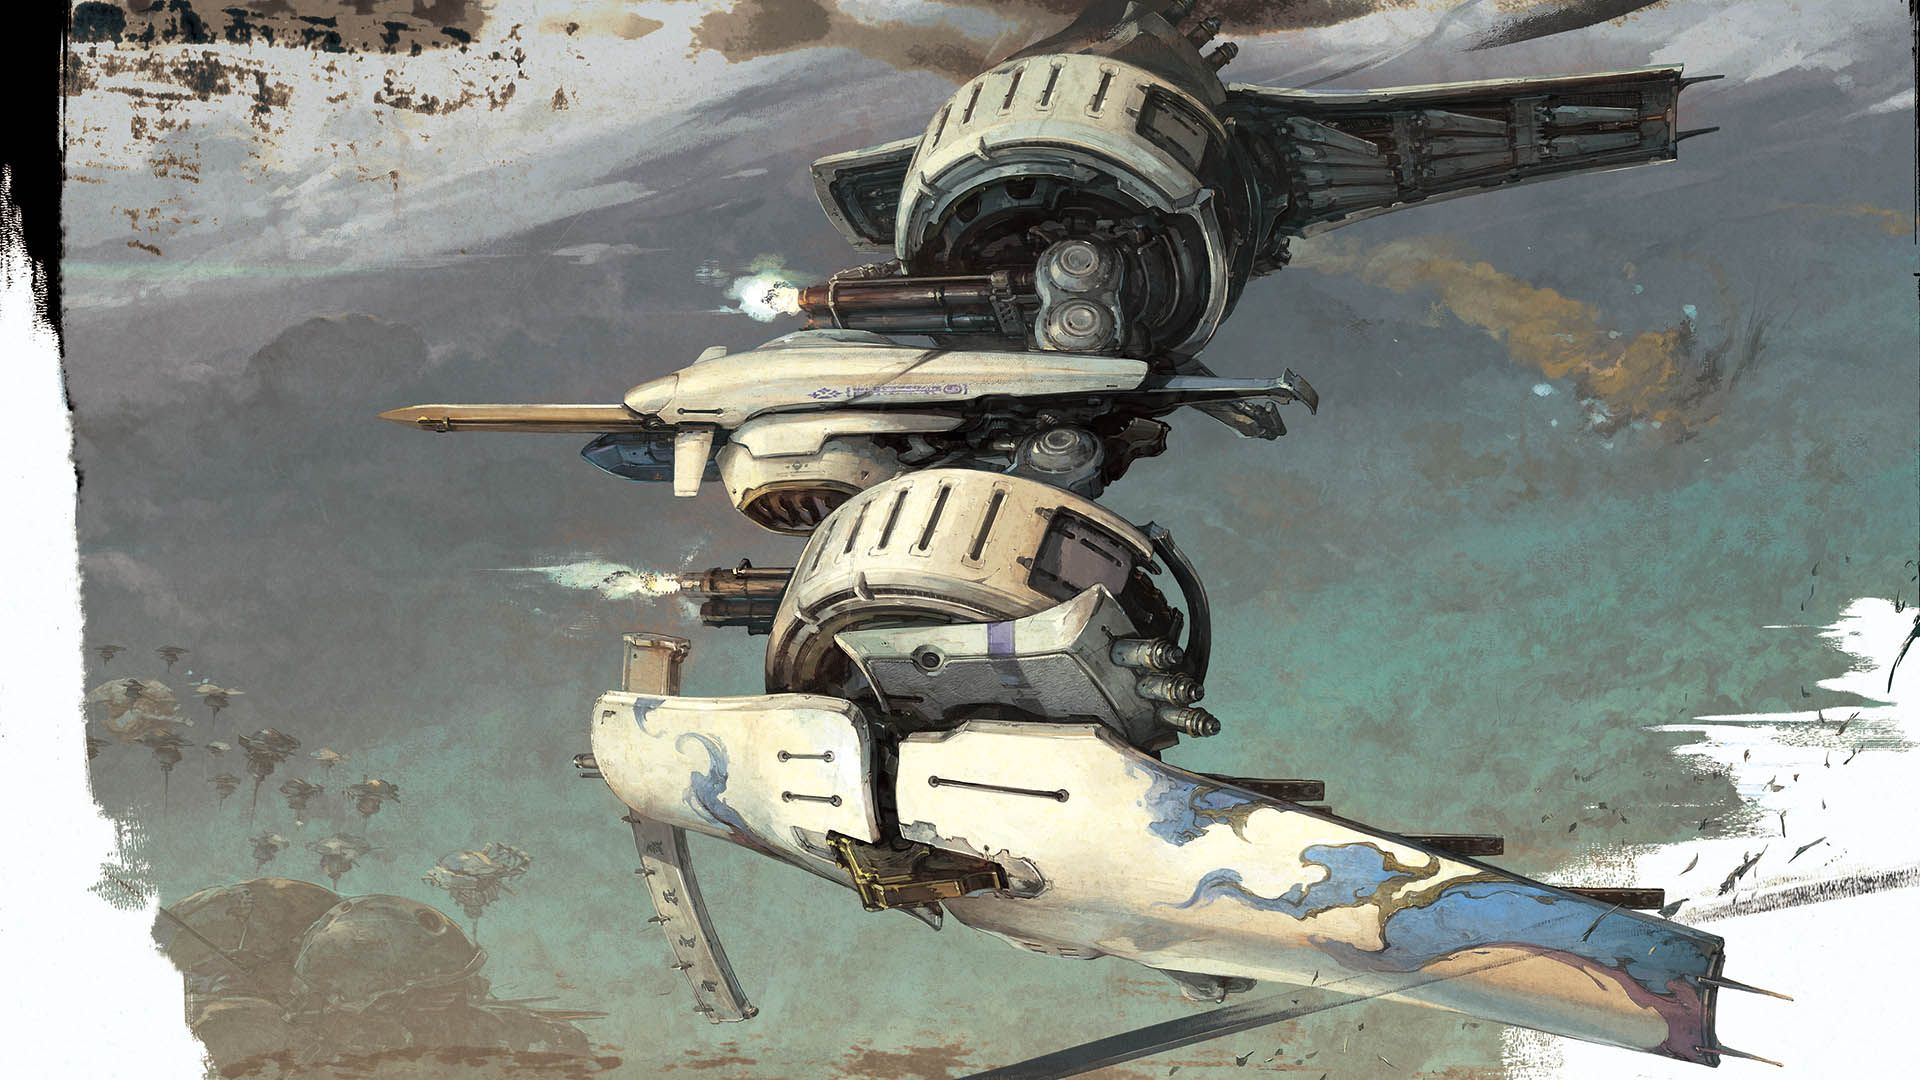
\includegraphics[width=1\textwidth]{Ikagura}
\caption{\label{fig:art}Art from Ikagura(1998)}
\end{figure}

\begin{figure}
\centering
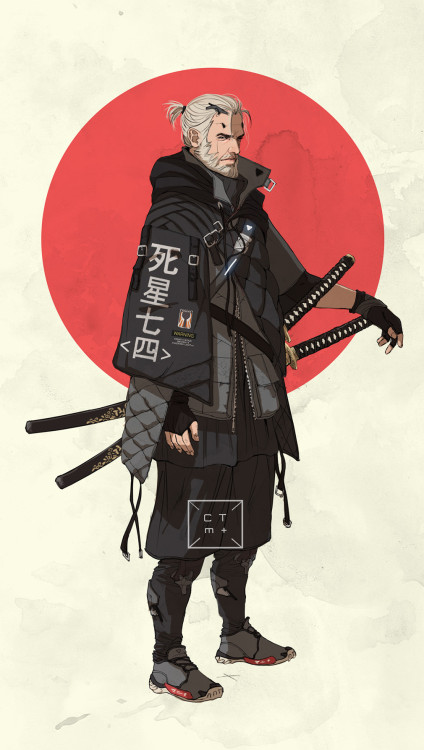
\includegraphics[width=0.5\textwidth]{Warrior}
\caption{Sci-fi warrior}
\end{figure}

\begin{figure}
  \centering
  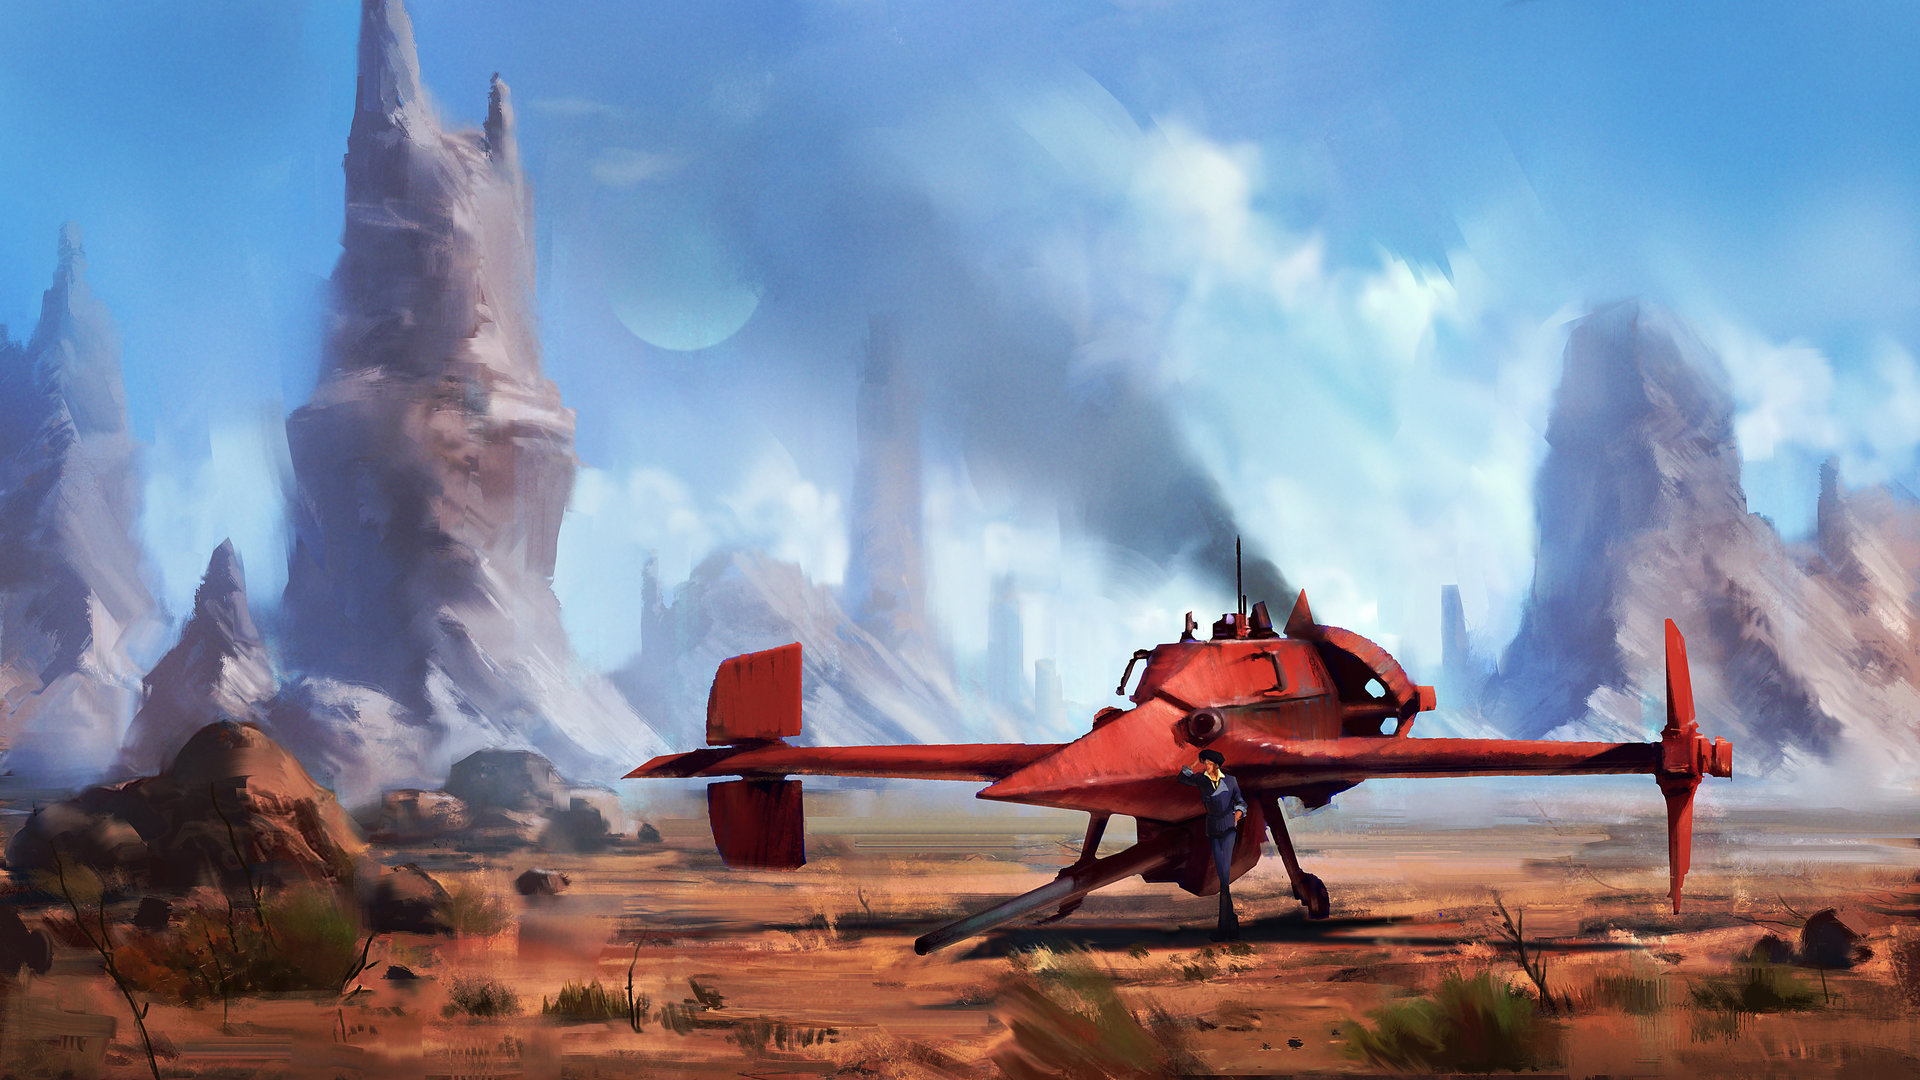
\includegraphics[width=1\textwidth]{Spaceship}
  \caption{'Cowboy Bebop' concept art}
  \end{figure}

\chapter{Gameplay and Game Setting}
be specific about the core game features 

\section{Story}
the story of the game

\section{World/Environment}
what is the settings of the game 

also, add here a map of your environment or a picture of your world if necessary

\section{User Interface}
who are the characters in the game?

\section{Main Objective}
what is the goal / main objective of the game?

\section{Core Mechanics}
very important section: what are the core mechanics? be specific

\section{Controls}
describe the controls of the game 
also, add here a controller diagram if necessary 

% ______________________
% chapter Front End
% ______________________


\chapter{Front End}
description of front end such as start screen, menu screens,..  

\section{Start Screen}

\section{Menus}

\section{End Screen}

% ______________________
% chapter Game Details
% ______________________


\chapter{Technology}
what technologies is the game designed for, what is the target platform, what technologies are used for the development? 

\section{Target Systems}
what platforms is the game designed for

\section{Hardware}
what hardware is needed to play the game? any additional interface? recommended controllers? 

\section{Development Systems/Tools}
please describe the tools you are using (game engine, art tools, ..) 

% ______________________
% chapter Game Details
% ______________________


\chapter{Topic and Inclusion }

describe here how you plan to address the main topic (main theme) and the 

\section{Main Theme}
\section{Inclusion}

\subsection{Diversity}
\subsection{Accessibility}
\subsection{Humanity}

% ______________________
% chapter Game Details
% ______________________

% ______________________
% chapter Game Details
% ______________________


\chapter{Timeline}

planned schedule 

\begin{table}[h]
\centering
\begin{tabular}{|l|l|l|}
\hline
Milestone & Description & Date \\\hline
& Official Start Date & 01.12.... \\
1 & Milestone Description ..  & 01.12.... \\
2 & Milestone Description ..  & 01.01.... \\
3 & Milestone Description ..  & 01.03.... \\
& End of Project & 01.04.... \\
\hline
\end{tabular}
\caption{\label{tab:schedule}Example Schedule.}
\end{table}


% ______________________
% chapter Game Details
% ______________________


\chapter{Team and Credits}

most important - who are you, who takes what role? 

e.g. :
Project Management: \\
Programming: \\ 
Art: \\ 
Design: \\ 

Additional Credits (e.g. sources of art, audio,.. ) 

%\todo[inline, color=green!40]{This is an inline comment.}

%\bibliographystyle{alpha}
%\bibliography{sample}

\end{document}